\documentclass[12pt]{article}
\usepackage{epsfig}
\usepackage{fullpage}
\usepackage{times}
\usepackage{comment}

\def\TA{Yu Chuan}
\def\InstructorMail{\texttt{nolan@stat.berkeley.edu}}
\def\TAMail{\texttt{s133@stat.berkeley.edu}}

\def\SFunctionRef#1{\textbf{#1}}
\def\SFunction#1{\textbf{#1}}
\def\Rpackage#1{\textit{#1}}

\begin{document}

\noindent
\textbf{Stat 133, Fall 04 \\
Homework 5: Ad Hoc Network Simulation\\
Due:  Wednesday, 17 Nov}

\medskip

Wireless networks are all around us.  Cell phones communicate with a
base-station to send and receive calls.  Calls are relayed from
base-station to base-station as the cell phone moves away from one and
closer to another.  A new idea of organizing networks is to avoid the
need for a central base-station that coordinates communications.
Instead, messages are relayed by ``hopping'' from one node to the next
to the next until it reaches its destination.  In other words, one can
send a message by using other devices in the network to relay the
message to the next device, and so on.  These are called \textit{ad
 hoc} networks because there is no centralized node or fixed
structure or topology for the network. Instead, devices can move over
time, and dynamically enter and exit the network.  And so the route a
message takes from one device to another depends on the other nodes.

Ad hoc networks are very promising and becoming important.  At their
most immediately practical, ad hoc networks can allow nodes outside of
a regular network to communicate by piggy-backing off of nodes within
the network.  Think of driving along and being between base-stations
and so your cell phone call would be dropped. But because of ad hoc
networks, your data is relayed through cell phones in other cars
closer to the base stations.  More ambituously, ad hoc networks might
be used in controlling traffic on highways by allowing cars
communicate with each other.

A very basic aspect of ad hoc networks that people need to understand
is how the communication and complete connectivity changes with
respect to the broadcasting power.  Increased power levels allow one to
send a message over a larger distance. 

\begin{itemize}
\item Start by generating a basic ad hoc network.  Place $75$ nodes 
 at random on the $2$-dimensional grid shown in Figure~\ref{contourPlot}, 
 where the node density is proportional to the function shown in 
 Figure~\ref{perspPlot}. Note the area of interest includes a ``river"
 where the density of nodes along the river is higher, except for 
 locations in the river and along the banks of the river. 
 This density function is supplied as an R function called 
\SFunctionRef{nodeDensity}. A vector of $x$ and a vector of $y$ coordinates 
 are taken as inputs to the function, and the return value is a vector
 of values that are proportional to node density at the $(x, y)$ pairs. 

\item Search over different power levels and determine whether the nodes are 
connected or not for the various power levels.  
Remember that for the set of nodes to be connected means that
it is possible for any two nodes to communicate by having a message
travel along nodes that are within broadcasting distance of each other.
If the power level is very high then all nodes will be able to broadcast
directly to each other. On the other hand, if the power level is too low
then a node may not be able to connect to any other node, or the nodes may
form two disjoint connected subsets. 
We are interested in finding the smallest power level that leads to a 
connected network. We assume here that power level is proportional
to the radius, $R$, of a circle centered on the node, and two nodes are 
in direct communication if the distance between them is less than $2R$.

\item How does the value of $R_c$, the smallest radius such that the
network is connected, change with different node configurations?
Repeat the above process of finding $R_c$ for 1000 random
node configurations generated according to the node density in 
Figure~\ref{perspPlot}. Explore the distribution of $R_c$. 
Is it symmetric, long tailed, similiar to any of the ``standard"
dositributions (normal, log-normal, expoenential, gamma, etc.)
Plot the network of connected points for four of your 1000 node 
configurations corresponding roughly to the min, median, mean, 
and maximum values of $R_c$. 

\end{itemize}

Functions that you may find helpful for this homework:
\SFunction{.Random.seed}, \SFunction{runif},
\SFunction{eigen}, \SFunction{which}, \SFunction{expand.grid},
\SFunction{contour}, \SFunction{dist}.

More information about how to determine whether a set of nodes
are connected for a particular power level will be available 
on the website soon.

You are to turn in your code, the \textit{random seed} used in your 
simulation (saved in a .rda file -- the seed must be unique to you), 
a description of the distribution of $R_c$ including one plot, 
and four plots of connected networks for the four values of $R_c$ 
mentioned above.

\begin{comment}
\begin{figure}
\epsfig{file= contourRiver.pdf, width=6.5in} 
\caption{Contour plot of the region of interest. The contours are proportional
to the density of nodes.}
\label{contourPlot}
\end{figure}

\begin{figure}
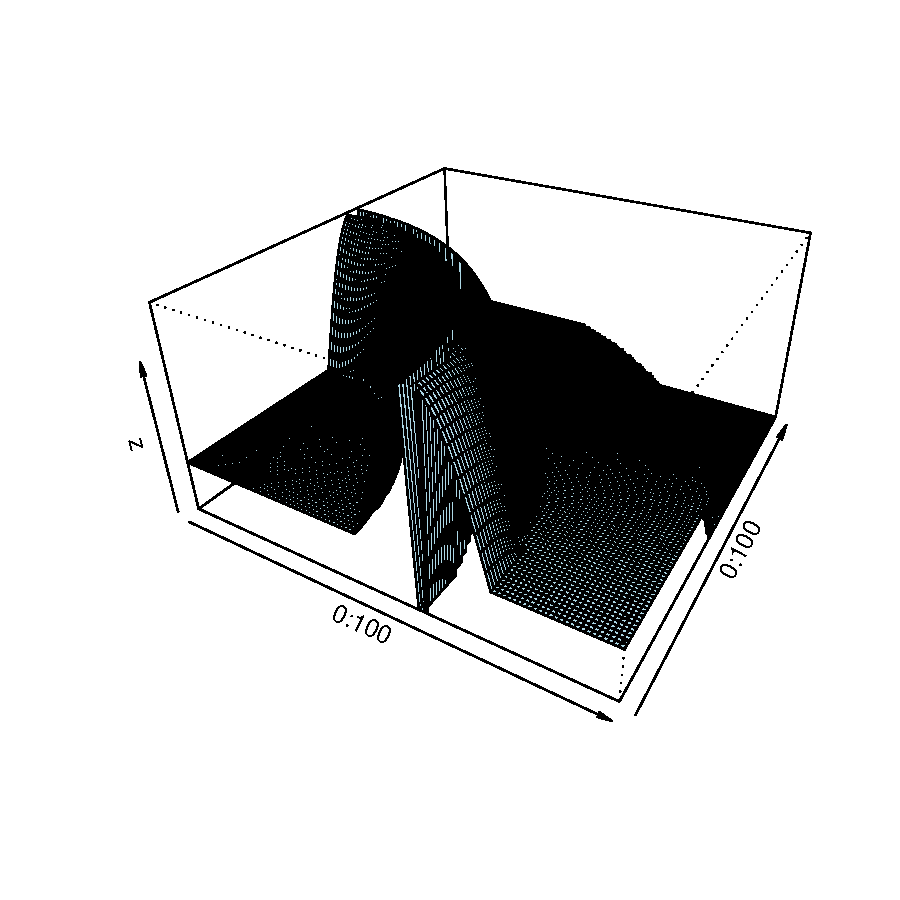
\epsfig{file=perspRiver, width=6.5in}
\caption{A three-dimensional perspective plot of the region of interest. 
Note that the river curves through the center of the region and no nodes
are located near the river.}
\label{perspPlot}
\end{figure}
\end{comment}

\end{document}
